\section{Cyber-spoofing simulation}
\label{sec:spoofing}
\subsection{Altering pseudoranges}
\label{subsec:altering_pseudoranges}
As a first experiment with our cyber-spoofing emulation, we operated on the logs collected in \ref{sec:opensky}. We chose to spoof our location 1 Km away from the real one, at the same altitude, of coordinates [45.0487414 N, 7.6682227 W]. The spoofing process computes, for each satellite in sight, the difference in the pseudorange that would be observed between the true location and the spoofed location; it then derives satellite-dependent time delays, which it adds to each log entry from that satellite.
In our setting, spoofing starts at $t = 150$ s, exactly in the middle of the logs collection period. 
\subsubsection{Effects on raw measurements}
\label{subsec:effects_raw_meas}
We were expecting both a sudden jump in the pseudoranges and a visible spike in the middle of the PRRs (when computed at runtime as a ratio of deltas, rather than being parsed from the logs). However, we observed that plotting PR amplitudes over time is not enough to visually notice the introduced difference while visualizing the behavior of more curves at once. 

Instead, considering only how the PR changes from their initial values, the jump is more evident. In fact, given that the receiver was standing still while collecting GNSS data, the plotted curves will be straight lines with a fairly stable slope while spoofing is not active, due to the natural movement of the SATs. By plotting only the slopes of those curves over time, which are a fair approximation of the PRRs, we see how the SAT-specific deltas added to the pseudoranges translated into a visible spike in each of the curves at $t = 150$ s (fig. \ref{fig:spoofing_no_delay_prrs}). This pulse-shaped alterations are far more readable to the eye and at the same time suggest that the absolute modifications over the pseudoranges were rather small. 

\begin{figure}[H]
    \centering
    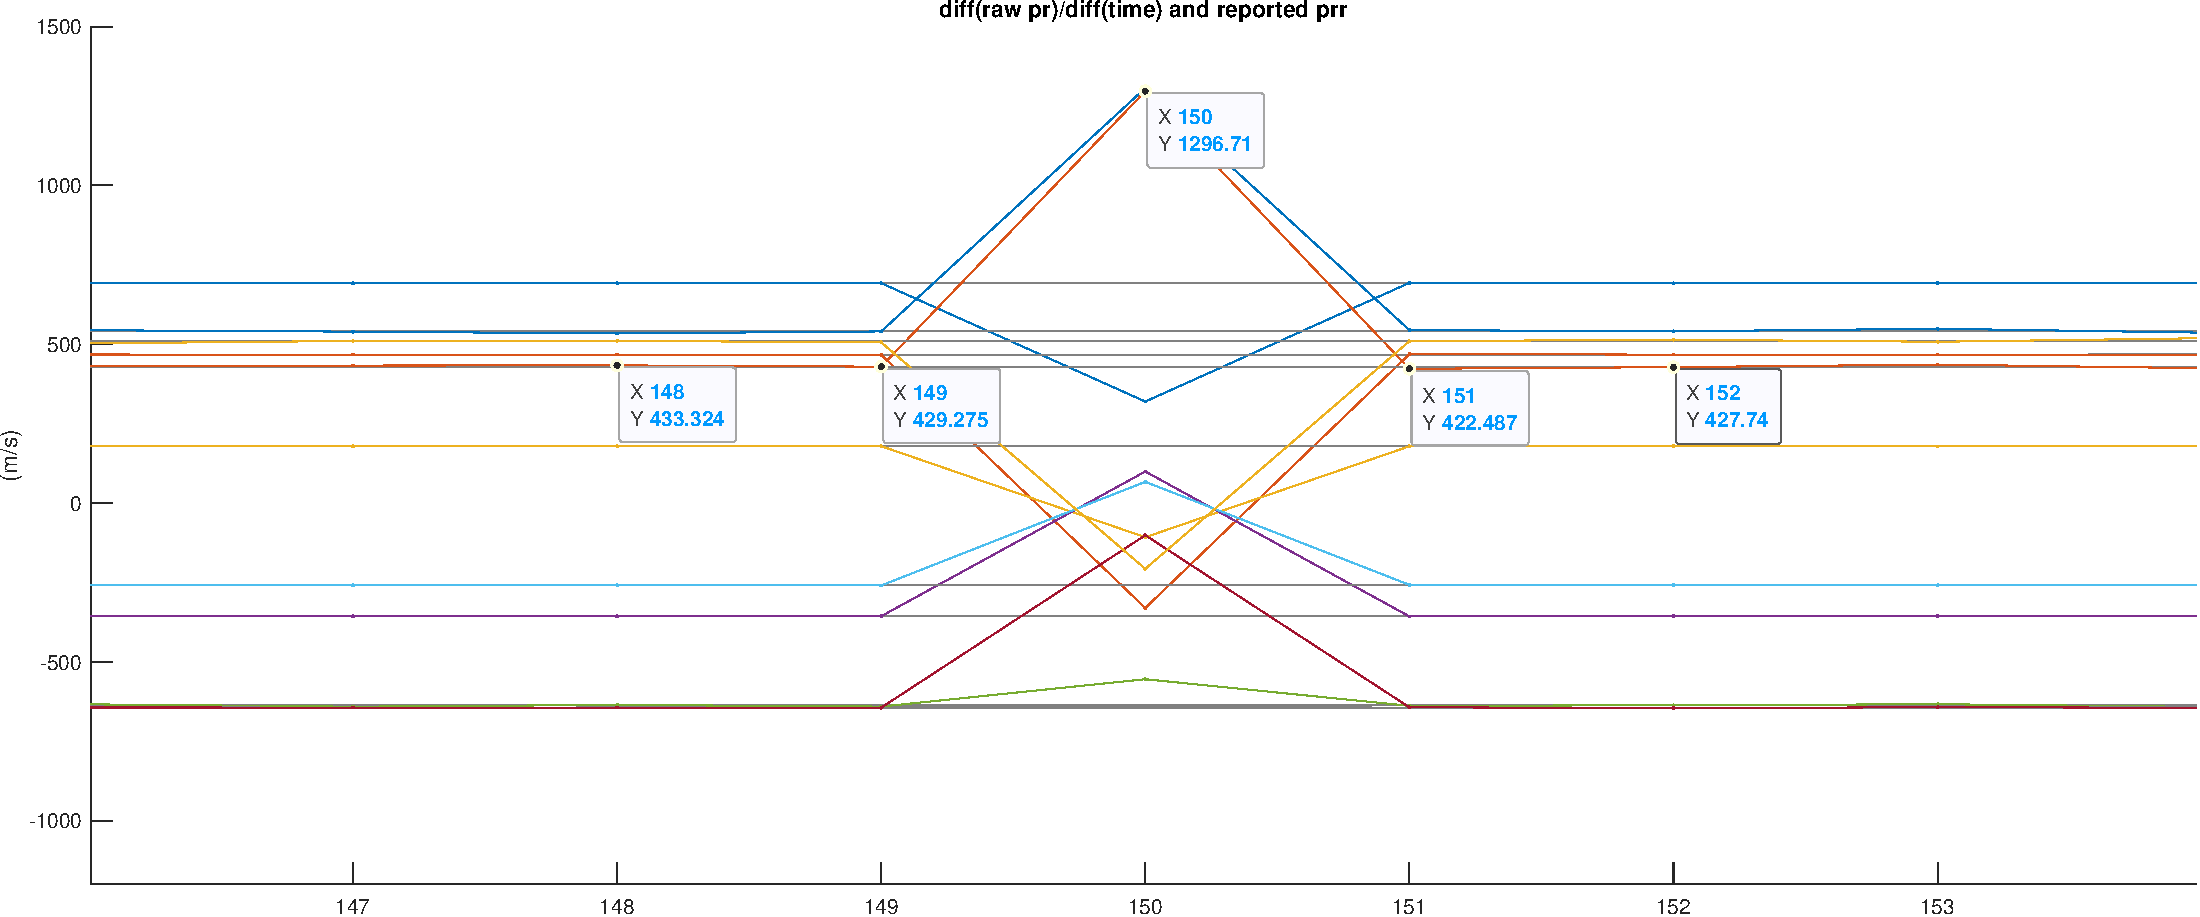
\includegraphics[width=0.75
    \linewidth]{images/1KM_spoofing_prr_of_sat_19}
    \caption{Pseudorange rates computed as ratios of deltas, or slopes of PR change from initial value over time. Tooltips show data about satellite 19.}
    \label{fig:spoofing_no_delay_prrs}
\end{figure}

Let's focus on SAT 19. Its pseudorange was about $2.25\cdot 10^7$ m during the whole logs collecting operation (fig. \ref{fig:pseudoranges_opensky}), and it was one among the most affected satellites by our spoofing. Its PR was also naturally changing due to the satellite moving, with a slope of about 430 m/s; the spoofing introduced a spike of about 1300 m/s at $t = 150$ s.

We can conclude that to trick the positioning algorithm into a location that was 1 Km away from the real one, each pseudorange has been altered by at most 0.00004\% of the value they had a second before the spoofing started. This really enhances our perspective on how the GNSS receivers rely on the smallest variations in the signal reception times to produce their outputs.

\subsubsection{Effects on PVT solution}
\label{sec:fratm}
While the most obvious effect of the spoofing simulation is the sudden change in positioning (fig. \ref{fig:pos_spoofed_no_delay}), the effects on the velocity states surely deserve attention. In fact, it's clear how velocities do not correspond to the ratios between the point-to-point distance and the time between two epochs, otherwise the velocity plots would present a visible spike in the middle, just like the plot of pseudoranges rates (fig. \ref{fig:spoofing_no_delay_prrs}).

Instead, velocities are being computed by exploiting the Doppler shift phenomenon \cite{psuDopplerShift2025}, because of which the signals from SATs are perceived by the receiver at slightly different frequencies, depending on the relative motion between the SAT and the receiver. Our receiver catched these subtle frequency shifts and autonomously derived PRRs (which here are to be interpreted as relative velocities between the receiver and the specific SAT) that we can find in the log entries (fields \textit{PseudorangeRateMetersPerSecond} and \textit{PseudorangeRateUncertaintyMetersPerSecond}). 

The MATLAB tool \cite{gpsMeasurementToolsCodebase} we used for the analysis has exploited those values, which our spoofing algorithm did not modify in any way, to estimate the velocity of the receiver; in particular, the WLS solver had to compensate the fact that in our new position we still had the previous relative velocity with respect to each of the SATs, which it did by tweaking the velocity estimates in both amplitude, direction and variance. This behavior justifies what we see in fig. \ref{fig:spoofing_velocities_no_delay}.

\begin{figure}[H]
    \centering
    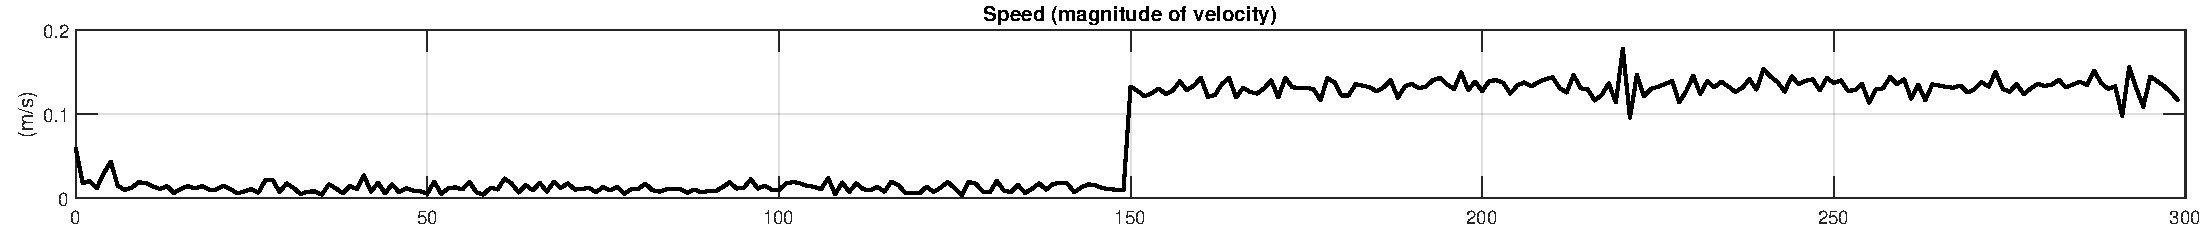
\includegraphics[width=1.00
    \linewidth]{images/spoofing_velocities_no_delay.pdf}
    \caption{Velocity states over time after spoofing}
    \label{fig:spoofing_velocities_no_delay}
\end{figure}

\subsection{Spoofing detection}
During the various tests we conducted, we made an attempt to identify methodologies for detecting ongoing cyber-spoofing activities.
% It should be noted that the following analysis is not highly precise, as the spoofing technique employed by the MATLAB tool \cite{gpsMeasurementToolsCodebase} differs from those typically used in real-world scenarios. Specifically, it operates by "falsifying" already recorded GNSS logs so that the resulting calculations return a spoofed position. In this context, certain warning signs can be identified. 
\subsubsection{Spikes in the runtime-computed pseudorange rates} 
\label{sec:boh}
From the analysis of the pseudorange rates graph, not only we see how the computed PRRs differ from the logged ones (the gray curves), but we also observe distinctive spikes, which occur when the PR value changes abruptly from one epoch to the next (fig. \ref{fig:spoofing_no_delay_prrs}).
When the spoofed location is far enough, the magnitude of the spike stands out clearly from the background noise, facilitating detection. 
% \colorbox{red}{TODO: inserire grafico picco derivata in relazione al rumore di fondo}

Moreover, since our spoofing technique involves adding deltas to all visible satellites starting from a selected timestamp, the spikes present themselves simultaneously, which allows to distinguish the spoofing event even in the case of spikes of lower amplitude. 
% \colorbox{red}{TODO: inserire grafico picco derivata visibile contemporaneamente su più satelliti}. 
\subsubsection{Inconsistent velocity states}
As previously mentioned, the spoofing emulation introduces anomalies in the velocities (\ref{sec:fratm}).
% To explain this more precisely: GNSS receivers are capable of estimating the velocity of the user not only through changes in position over time, but also through analysis of the Doppler shift — the variation in the frequency of the signal received from each satellite.
% If a satellite moves toward the receiver, the signal’s frequency appears slightly higher than its nominal value; conversely, if it moves away, the frequency appears lower.
% By measuring these frequency shifts for multiple satellites, the receiver can reconstruct the complete 3D velocity vector of the device with high accuracy. This Doppler-based velocity is independent from the pseudorange-based position calculation.

% However, when spoofing is introduced using the Google tool, this mechanism breaks. The spoofing affects only the pseudorange data (i.e., the perceived position), while the frequencies and Doppler shifts remain unchanged and still reflect the true physical position of the receiver.
% This inconsistency leads to the detection of sudden and unrealistic velocity changes. 

For instance, the sudden increase in speed that the WLS solver introduces when the spoofing starts may not be wide enough to justify the position shift. In our example, the spoofed position was 1 Km away from the real one, but velocity peaked at less than 0.2 m/s, instead of showing a spike reaching 1 Km/s in $t = 150$ s (which would have have been unrealistic nonetheless, in terms of acceleration) (fig. \ref{fig:spoofing_velocities_no_delay}).

A more complex cyber-spoofing strategy, which would also alter the pseudorange rates, would probably cancel this behavior, but is also likely to be detected by searching for sudden changes in the PRRs themselves, or by correlating such values to data taken from other sensors the system is equipped with, such as accelerometers.
\subsection{Adding time delay}
\label{subsec:time_delay}

Starting the spoofing attack at $t = 150$ s and using the previously spoofed position, we set the variable \textit{spoof.delay} = 0.003, meaning a 3 ms delay. Essentially, the script now not only will modify the signal reception times by adding SAT-dependent delays, but also simulate that they all were received 3 ms later than they actually were.
The change in delay creates a scenario very similar to a meaconing attack. In fact, the only difference here is that we are applying an additional common delay to all the satellite signals, that will be incorporated into the receiver's clock bias. This bias will be estimated and accounted for during the calculation by the WLS solver. The resulting change in the bias due to this delay is evident in figure \ref{fig:spoofing_clock_bias_with_delay}.
\begin{figure}[H]
    \centering
    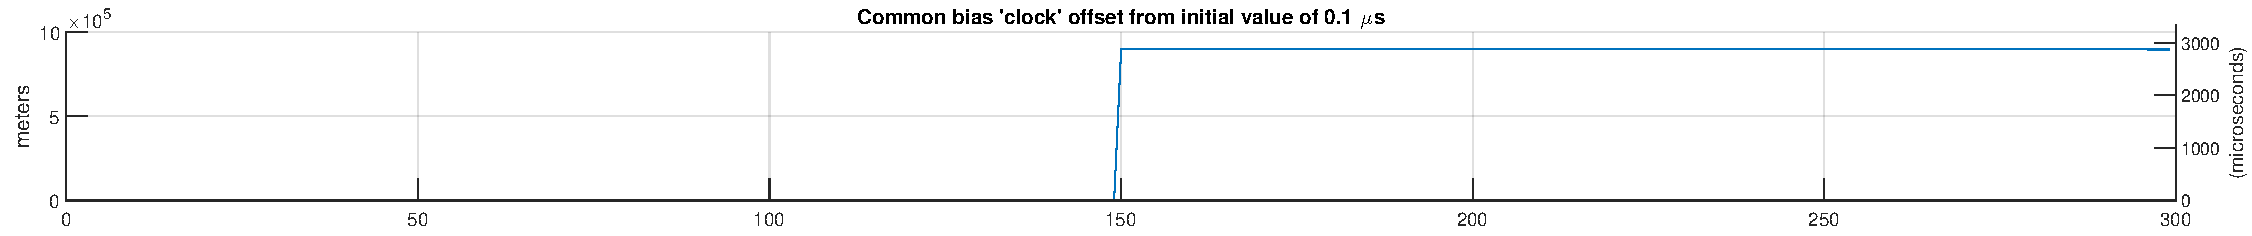
\includegraphics[width=1.00
    \linewidth]{images/clock_bias_with_delay.pdf}
    \caption{Common user clock bias after spoofing with additional delay}
    \label{fig:spoofing_clock_bias_with_delay}
\end{figure}
Since this delay change only affects the clock bias, the position will still be calculated correctly. However, unlike the simple spoofing attack, where a very small change in pseudoranges could falsify the position by 1 km, we now observe a larger shift in the pseudoranges, which take on much larger values. This behavior, which we discussed in the first HW clock discontinuity scenario, is due to the growing clock bias, now caused by the delay, which wasn't properly corrected in the graph (fig. \ref{fig:spoofing_pseudoranges_with_delay}).
\begin{figure}[H]
    \centering
    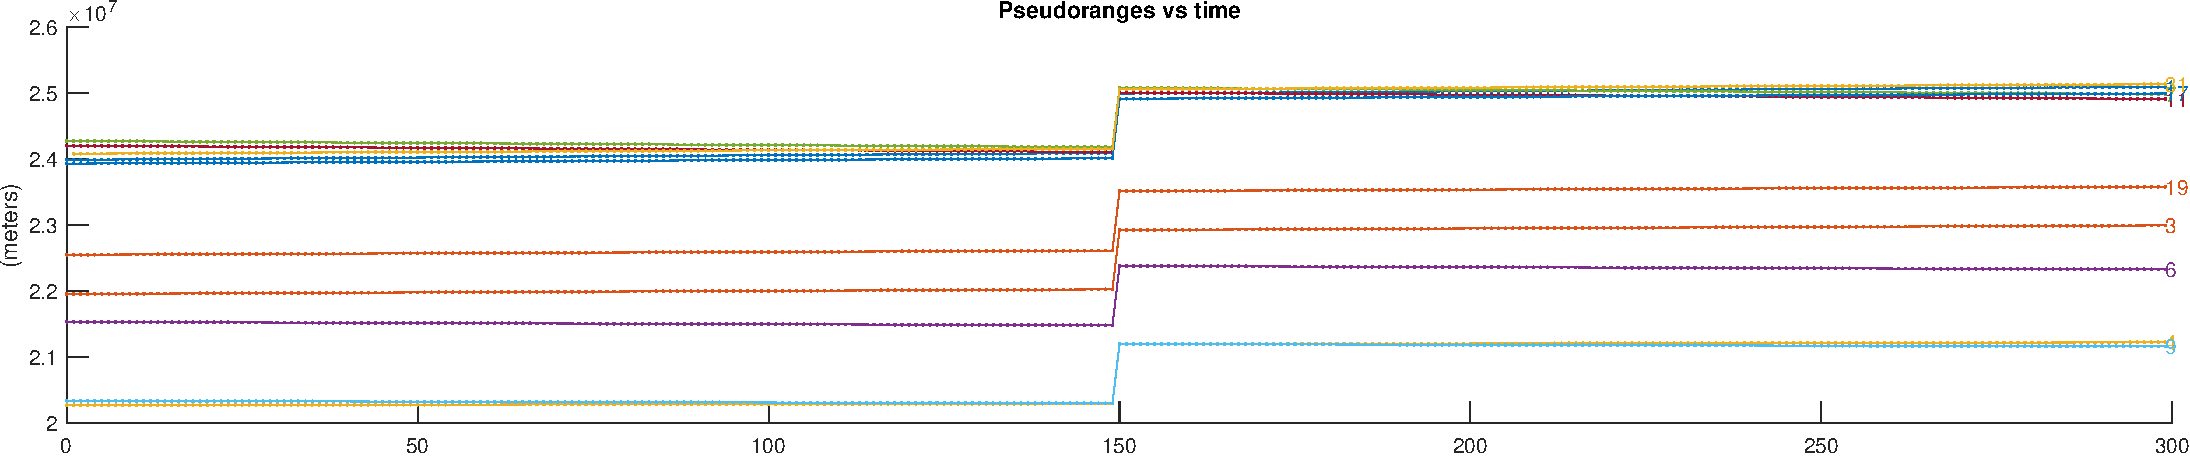
\includegraphics[width=1.00
    \linewidth]{images/spoofing_prs_change_due_to_delay.pdf}
    \caption{Pseudoranges vs. time, after spoofing with  additional delay}
    \label{fig:spoofing_pseudoranges_with_delay}
\end{figure}